\chapter{Einleitung}

Bereits 1966 hat Joseph Weizenbaum mit ELIZA am \acf{MIT} ein Programm geschaffen, das Strukturen in menschlicher Sprache erkennen, verstehen und auf diese antworten kann, den ersten Chatbot sozusagen.\footcite[Vgl.][o. \pno]{Weizenbaum_1966}

Auch in der heutigen Gesellschaft ist diese Funktionalität gefragter denn je. Besonders auf Unternehmenswebsiten oder Online-Shops sind immer häufiger Chatbots anzutreffen und die Kunden stehen dem, wie in \autoref{fig:bewertungchatbots} zu sehen ist vermehrt neutral bis positiv gegenüber.
\footcite[Vgl.][50]{Groetz_2018_Sprich_mit_mir}


\begin{figure}[H]
  \centering
  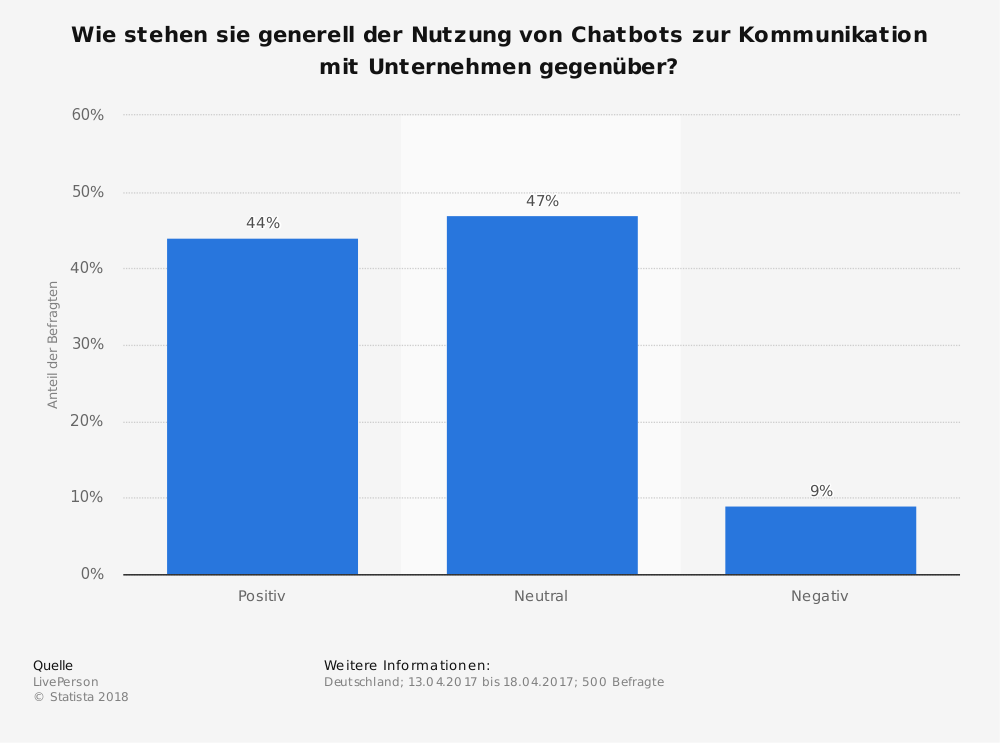
\includegraphics[width=0.6\textwidth]{Anhang/2018_stat_bewertung_chatbots}
  \quelle[o. \pno]{Statista_2019_Bewertung_Chatbots}
  \caption{Bewertung von Chatbots}
\label{fig:bewertungchatbots}
\end{figure}

Auch in Privathaushalten halten Chatbots in Form von Sprachassistenten wie \textit{Amazon Alexa} oder \textit{Google Home} Einzug und an jedem aktuellen Windows-Computer kann mittlerweile \textit{Microsoft Cortana} genutzt werden. Im Rahmen der Heimautomatisierung können so Heizung oder Licht per Sprachinteraktion mit Sprachassistenten bzw. Chatbots gesteuert werden. \footcite[Vgl.][o. \pno]{Kuhn_2015_Sprachassistenten}

% \todo{Puppet Bot, Sprachassistenten im weiteren Sinne Bots}
Da ist es naheliegend, dass man diese Technologie auch im Bereich der Softwareentwicklung oder des Rechenzentrumsbetriebs zur Automatisierung verwenden möchte. GitHub hat dies 2013 erkannt und mit der Vorstellung des Chatbots \textit{Hubot} den Begriff ChatOps, also die Integration eines Chatbots in eine Toolchain oder einen Prozess, geprägt. \footcite[Vgl.][o. \pno]{GitHub_2013_Chatops}

Auch das bekannte, an Unternehmenskunden gerichtete Chat-Tool \acf{Slack} bietet die Möglichkeit, Chatbots zu entwickeln und somit an die eigene Arbeitsumgebung anzupassen. \footcite[Vgl.][o. \pno]{Koeltzsch_2019_Slack}


\section{Umfeld}
Der Autor ist beim \acf{IVZ} beschäftigt, einer Kooperation aller Rundfunkanstalten der \acf{ARD}, sowie Deutschlandradio und \acf{DW} mit Hauptsitz im \acf{rbb}.
Es wurde 1993 als öffentlich-rechtliche Verwaltungsgemeinschaft gegründet und beschäftigt etwa 200 Mitarbeiter an mehreren Standorten.\footcite[Vgl.][o. \pno]{ARD_2018_IVZ}\\
Das \acs{IVZ} bietet seinen Kunden zentral, \acs{ARD}-weite Rechenzentrumsdienstleistungen, wie z. B. SAP oder Archive (Video, Audio, Text) an. Unternehmensweit wird ein Chat-Tool zur Teamkommunikation eingesetzt.


\section{Ziel der Arbeit}
Ziel der vorliegenden Arbeit ist es, zu evaluieren, ob die Einführung einer ChatOps Schnittstelle zur \acf{CMDB} die Arbeit der Mitarbeiter im Rechenzentrumsbetrieb beim Umgang mit dieser erleichtert und angenehmer macht. Bestimmte Aktionen der \acs{CMDB} können in diesem Szenario aus einem Chat-Tool heraus aufgerufen werden und bieten eine Alternative zum Standardweg per Website oder Client. Durch die Befragung von Experten in diesem Gebiet soll beantwortet werden, ob der Einsatz von ChatOps in diesem Zusammenhang nutzenbringend ist.

%"Lässt sich die Arbeit der RZ Mitarbeiter beim Umgang mit der CMDB durch ChatOps erleichtern?"

\section{Abgrenzung}
Nicht Bestandteil dieser Arbeit ist die Evaluierung von ChatOps im Allgemeinen, sowie der Nutzen von ChatOps im gesamten Tätigkeitsspektrum des Rechenzentrumsbetriebs. Der Fokus liegt lediglich auf der Verwendung der CMDB. Außerdem soll nicht der gesamte Funktionsumfang einer \acs{CMDB} betrachtet werden, sondern nur die Komponenten und Funktionen, die im Tagesgeschäft des Rechenzentrumsbetriebs häufig verwendet werden.

\section{Vorgehensweise}
%In \autoref{empg} werden die relevanten empirischen Methoden zur Erforschung des Themas vorgestellt, die Voraussetzung zum Verständnis von \autoref{AnfA} sind.
In \autoref{theg} werden die für das Verständnis der Thematik notwendigen Fachbegriffe eingeführt, erläutert und in einen Zusammenhang gesetzt. In \autoref{AnfA} wird eine Anforderungsanalyse durchgeführt, um die im Arbeitsalltag am meisten genutzten \acs{CMDB} Funktionen zu ermitteln und herauszufinden, in welchen Fällen eine ChatOps Umsetzung möglich und sinnvoll ist. Die Anforderungen werden mithilfe von Experteninterviews ermittelt, wobei die Analyse der Transkripte nach der Methode von Meuser und Nagel erfolgt.\\
In \autoref{Praxis} wird ein Chatbot entworfen und die Interaktion mit der bestehenden \acs{CMDB} beschrieben.
Abschließend wird in \autoref{Fazit} ein Fazit gezogen, es wird aufgrund der in dieser Arbeit gewonnenen Erkenntnisse geschlussfolgert, welchen Nutzen und Vorteil ChatOps im betrachteten Kontext bietet. Darüber hinaus wird ein Ausblick gegeben, wie ChatOps sich in Zukunft entwickeln könnte und in welchen Gebieten (im Rechenzentrum und darüber hinaus) es ebenfalls Fuß fassen könnte.

% \section{Über diese Arbeit}
Diese Arbeit ist in \LaTeX~gesetzt. Die Versionierung wurde mit Git vorgenommen.
